% ------------------------------------------------------------------------------
% TYPO3 Version 10.1 - What's New (French Version)
%
% @license	Creative Commons BY-NC-SA 3.0
% @link		http://typo3.org/download/release-notes/whats-new/
% @language	French
% ------------------------------------------------------------------------------

\section{Changements pour les intégrateurs}
\begin{frame}[fragile]
	\frametitle{Changements pour les intégrateurs}

	\begin{center}\huge{Chapitre 2~:}\end{center}
	\begin{center}\huge{\color{typo3darkgrey}\textbf{Changements pour les intégrateurs}}\end{center}

\end{frame}

% ------------------------------------------------------------------------------
% Feature | 89102 | Read settings for sites from <config>/sites/<siteIdentifier>/settings.yaml
%
%\begin{frame}[fragile]
%	\frametitle{Changements pour les intégrateurs}
%	\framesubtitle{Site-specific Settings (1)}
%
%	% decrease font size for code listing
%	\lstset{basicstyle=\smaller\ttfamily}
%
%	\begin{itemize}
%		\item A YAML file can provide site specific variables independent of the current context.
%
%		\item Place the file in the site configuration folder:\newline
%			\texttt{<config>/sites/<siteIdentifier>/settings.yaml}
%
%		\item For example:
%
%\begin{lstlisting}
%Vendor:
%   MyExtension:
%      storagePid: 1
%      limit: 15
%\end{lstlisting}
%
%	\end{itemize}
%
%\end{frame}
%
% ------------------------------------------------------------------------------
% Feature | 89102 | Read settings for sites from <config>/sites/<siteIdentifier>/settings.yaml
%
%\begin{frame}[fragile]
%	\frametitle{Changements pour les intégrateurs}
%	\framesubtitle{Site-specific Settings (2)}
%
%	% decrease font size for code listing
%	\lstset{basicstyle=\smaller\ttfamily}
%
%	\begin{itemize}
%		\item Settings can be accessed in TypoScript:
%
%\begin{lstlisting}
%plugin.tx_example.storagePid = {$Vendor.MyExtension.storagePid}
%\end{lstlisting}
%
%		\item Settings can also be accessed in PHP using the \texttt{Site} object:
%
%\begin{lstlisting}
%$settings = $site->getSettings();
%$storagePid = $settings['MyVendor']['MyExtension']['storagePid'];
%\end{lstlisting}
%
%	\end{itemize}
%
%\end{frame}

% ------------------------------------------------------------------------------
% Feature | 89227 | Ask for email address while installing TYPO3

\begin{frame}[fragile]
	\frametitle{Changements pour les intégrateurs}
	\framesubtitle{Adresse email administrateur}

	\begin{columns}[T]
		\begin{column}{.04\textwidth}
		\end{column}
		\begin{column}{.38\textwidth}

			La saisie d'une adresse email fait partie de la procédure d'installation.
			Cette adresse est utilisée pour le premier administrateur du backend.

			\vspace{0.2cm}

			L'option existe aussi dans l'action \textbf{Create Administrative User} du
			module de maintenance de l'outil d'installation.
			

		\end{column}
		\begin{column}{.58\textwidth}
			\vspace{-0.3cm}
			\begin{figure}
				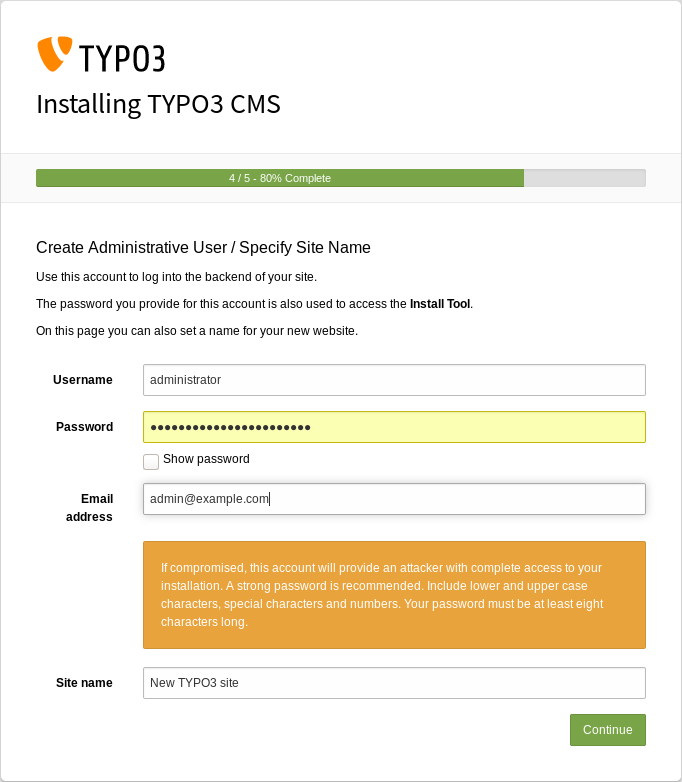
\includegraphics[width=0.70\linewidth]{ChangesForIntegrators/89227-EmailAddressDuringInstallation.png}
			\end{figure}
		\end{column}
	\end{columns}

\end{frame}

% ------------------------------------------------------------------------------
% Feature | 89229 | Cache Preset for Settings in Maintenance Area

% TRANSLATORS, PLEASE BE AWARE:
% We already included this slide in the 10.0 What's New Slides! However, the
% feature #89229 was removed from the TYPO3 core shortly before version 10.0 was
% published. Therefore, you possibly don't need to translate this slide again
% (just copy the text from the previous What's New Slides (search for the term
% "Cache Storage Type" in file ChangesForIntegrators.tex).

\begin{frame}[fragile]
	\frametitle{Changements pour les intégrateurs}
	\framesubtitle{Type de stockage des caches (1)}

	\begin{itemize}

		\item TYPO3 fournit un système de cache flexible avec une configuration
				par défaut idéale dans la plupart des cas.
		\item Le type de stockage est configurable pour affiner les caches et
		augmenter les performances en fonction de l'environnement.

		\begin{itemize}
			\item Choisir le stockage en \textbf{base de données} pour un environnement classique
				ou si, par exemple, un système de fichiers réseau (NFS) est utilisé.
			\item Choisir le stockage sur le \textbf{système de fichiers} si, par exemple,
				une base de données distribuée est utilisée.
			\item Choisir des \textbf{paramètres de cache sur mesure} afin de configurer les types de stockage
				de façon indépendante.
		\end{itemize}

		\item Dans le cas d'installations plus complexes, des caches mémoire comme
			\href{https://redis.io/}{Redis (en)}
			ou
			\href{https://memcached.org/}{Memcached (en)} sont à étudier.

	\end{itemize}

\end{frame}

% ------------------------------------------------------------------------------
% Feature | 89229 | Cache Preset for Settings in Maintenance Area

% TRANSLATORS, PLEASE BE AWARE:
% We already included this slide in the 10.0 What's New Slides! However, the
% feature #89229 was removed from the TYPO3 core shortly before version 10.0 was
% published.
%
% On this slide, the path to the function in the backend needs to be adjusted:
% ADMIN TOOLS -> Settings -> Configuration Presets

\begin{frame}[fragile]
	\frametitle{Changements pour les intégrateurs}
	\framesubtitle{Type de stockage des caches (2)}

	\begin{itemize}

		\item Backend~: \textbf{ADMIN TOOLS} \ding{223}\hspace{0.1cm}\textbf{Settings} \ding{223}\hspace{0.1cm}\textbf{Configuration Presets}~:
		\end{itemize}

	\begin{figure}
		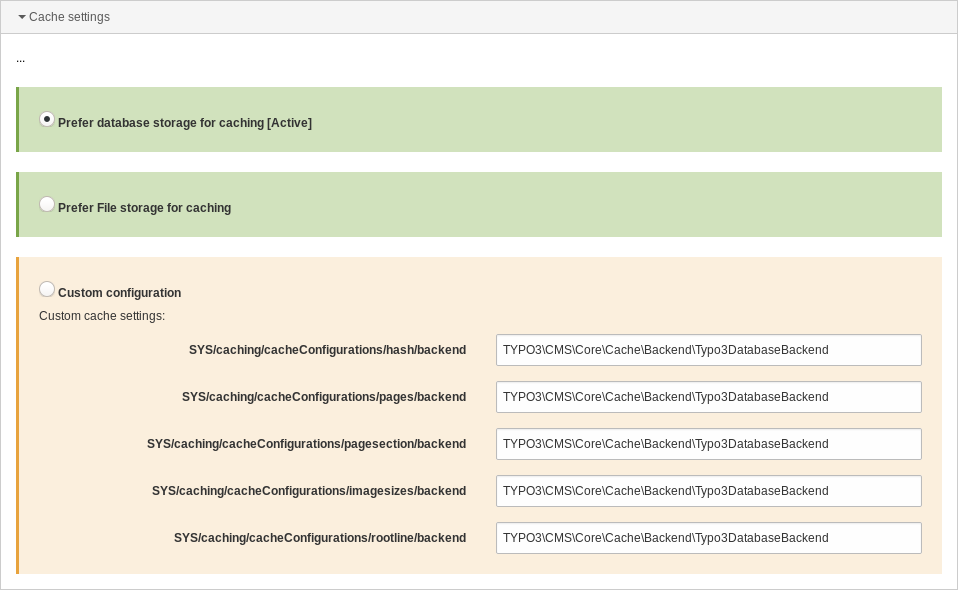
\includegraphics[width=0.60\linewidth]{ChangesForIntegrators/89229-CachePresetForSettingsInMaintenanceArea.png}
	\end{figure}

\end{frame}

% ------------------------------------------------------------------------------
% Feature | 89142 | Create site configuration if page is created on root level

\begin{frame}[fragile]
	\frametitle{Changements pour les intégrateurs}
	\framesubtitle{Configuration du Site}

	\begin{itemize}
		\item À la création d'une nouvelle page au niveau racine, une configuration
			de site standard est automatiquement générée.
		\item On peut donc créer un site TYPO3 rapidement.
		\item La configuration contient~:

			\begin{itemize}
				\item Un identifiant prédéfinit (i.e. \texttt{site-42-a1d0c6e83f})
				\item Un point d'entrée (i.e. \texttt{https://example.com/site-42})
				\item Une langue par défaut (i.e. \texttt{English})
			\end{itemize}

	\end{itemize}

\end{frame}

% ------------------------------------------------------------------------------
% Feature | 89090 | Reports for conflicting redirects

\begin{frame}[fragile]
	\frametitle{Changements pour les intégrateurs}
	\framesubtitle{Conflits de redirection (1)}

	\begin{itemize}
		\item Une commande Symfony est introduite pour la détection des redirections
			en conflit avec les URLs de page.
		\item Exécuter la commande CLI~:\newline
			\smaller
				(le paramètre optionnel \texttt{-}\texttt{-site} limite la vérification à un site spécifique)
			\normalsize
	\end{itemize}

	\begin{figure}
		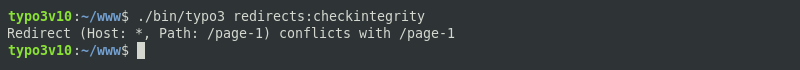
\includegraphics[width=0.90\linewidth]{ChangesForIntegrators/89090a-ReportsForConflictingRedirects.png}
	\end{figure}

	\begin{itemize}
		\item Cette commande est aussi disponible dans le planificateur~:
	\end{itemize}

	\begin{figure}
		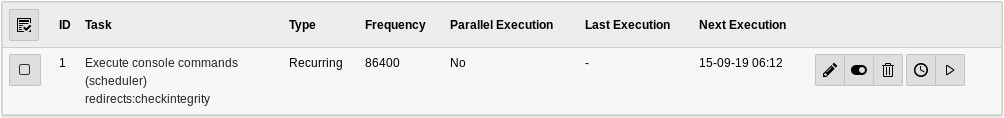
\includegraphics[width=0.90\linewidth]{ChangesForIntegrators/89090b-ReportsForConflictingRedirects.png}
	\end{figure}

\end{frame}

% ------------------------------------------------------------------------------
% Feature | 89090 | Reports for conflicting redirects

\begin{frame}[fragile]
	\frametitle{Changements pour les intégrateurs}
	\framesubtitle{Conflits de redirection (2)}

	\begin{itemize}
		\item La liste des conflits de redirections est aussi disponible dans le module Rapports~:
	\end{itemize}

	\begin{figure}
		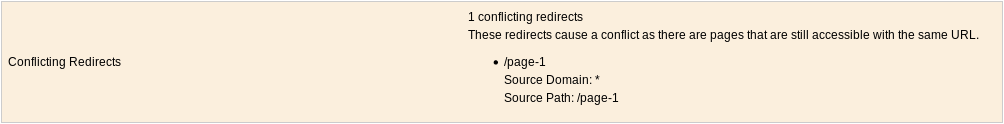
\includegraphics[width=0.90\linewidth]{ChangesForIntegrators/89090c-ReportsForConflictingRedirects.png}
	\end{figure}

	\begin{itemize}
		\item
			\small\textbf{Note~:}
				La commande doit être exécutée de nouveau pour réinitialiser la liste.
				Résoudre les problèmes (i.e. retirer la redirection) ne vide pas la liste.
			\normalsize
	\end{itemize}

\end{frame}

% ------------------------------------------------------------------------------
% Feature | 89010 | Introduce Site Configuration for Distribution Packages

\begin{frame}[fragile]
	\frametitle{Changements pour les intégrateurs}
	\framesubtitle{Distributions}

	% decrease font size for code listing
	\lstset{basicstyle=\tiny\ttfamily}

	\begin{itemize}
		\item Les distributions peuvent fournir leurs fichiers de configuration de site.

		\item Créer un dossier / fichier dans l'archive de la distribution comme suit~:\newline
			\texttt{Initialisation/Site/<siteIdentifier>/config.yaml}

		\item Comme les ressources, qui sont déplacées dans le dossier \texttt{fileadmin/},\newline
			les configurations de site sont déplacées dans le dossier \texttt{config/}.

		\item Si le répertoire cible existe déjà, aucun de changement de configuration n'est effectué.
	\end{itemize}

\end{frame}

% ------------------------------------------------------------------------------
% Feature | 88318 | Display Application Context in CLI

\begin{frame}[fragile]
	\frametitle{Changements pour les intégrateurs}
	\framesubtitle{Contexte d'application en CLI}

	\begin{itemize}
		\item Le contexte d'application actuel apparaît à côté de la version de
			TYPO3 dans les requêtes CLI~:
	\end{itemize}

	\begin{figure}
		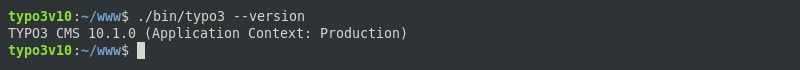
\includegraphics[width=0.90\linewidth]{ChangesForIntegrators/88318-DisplayApplicationContextInCli.png}
	\end{figure}

\end{frame}

% ------------------------------------------------------------------------------
% Feature | 87525 | Add api=1 option in VimeoRenderer

\begin{frame}[fragile]
	\frametitle{Changements pour les intégrateurs}
	\framesubtitle{Rendu des vidéos Vimeo}

	% decrease font size for code listing
	\lstset{basicstyle=\smaller\ttfamily}

	\begin{itemize}
		\item Le paramètre \texttt{api=1} des URLs Vimeo autorise les interactions
			avec l'API du lecteur (par exemple~: ajout de boutons de contrôle vidéo).
		\item Les intégrateurs peuvent déclarer ce paramètre de deux façons~:

		\begin{itemize}
			\item En TypoScript~:

\begin{lstlisting}
lib.contentElement.settings.media.additionalConfig.api = 1
\end{lstlisting}

			\item Dans Fluid en utilisant le ViewHelper Media~:

\begin{lstlisting}
<f:media
  file="{file}"
  alt="{file.properties.alternative}"
  title="{file.properties.title}"
  additionalConfig="{api: 1}"
/>
\end{lstlisting}

		\end{itemize}
	\end{itemize}

\end{frame}

% ------------------------------------------------------------------------------
% Feature | 86670 | Make default action in DragUploader adjustable

\begin{frame}[fragile]
	\frametitle{Changements pour les intégrateurs}
	\framesubtitle{Chargement de fichiers}

	% decrease font size for code listing
	\lstset{basicstyle=\smaller\ttfamily}

	\begin{itemize}
		\item Il est possible de configurer l'action par défaut lorsqu'on charge des fichiers
			à l'aide du glisser-déplacer du module de liste des fichiers.
		\item User TSConfig~:

\begin{lstlisting}
# Set default to replace:
options.file_list.uploader.defaultAction = replace

# Set default to rename:
options.file_list.uploader.defaultAction = rename

# Set default to cancel:
options.file_list.uploader.defaultAction = cancel
\end{lstlisting}

	\end{itemize}

\end{frame}

% ------------------------------------------------------------------------------
% Feature | 84250 | Separately enable / disable "Add media by URL" and "Select & upload files"

\begin{frame}[fragile]
	\frametitle{Changements pour les intégrateurs}
	\framesubtitle{Boutons des éléments média}

	% decrease font size for code listing
	\lstset{basicstyle=\tiny\ttfamily}

	\begin{itemize}
		\item Les boutons \textbf{«~Ajouter un média à partir d’une URL~»} et
			\textbf{«~Sélectionner et transférer des fichiers~»} sont activables
			/ désactivables indépendamment.
	\end{itemize}

	\begin{figure}
		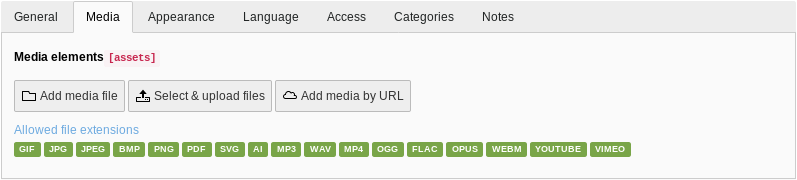
\includegraphics[width=0.75\linewidth]{ChangesForIntegrators/84250-EnableDisableMediaButtons.png}
	\end{figure}

	\begin{itemize}
		\item L'exemple ci-dessous montre comment cacher les deux boutons~:

\begin{lstlisting}
$GLOBALS['TCA']['pages']['columns']['media']['config']['appearance'] = [
  'fileUploadAllowed' => false,
  'fileByUrlAllowed' => false,
];
\end{lstlisting}

	\end{itemize}

\end{frame}

% ------------------------------------------------------------------------------
% Feature | 88441 | Show configuration of USER_INT objects in adminpanel

\begin{frame}[fragile]
	\frametitle{Changements pour les intégrateurs}
	\framesubtitle{Panneau d'administrateur}

	\begin{itemize}
		\item Le panneau d'administrateur inclus un panneau \textbf{USER\_INT} sous le module Info.
	\end{itemize}

	\begin{figure}
		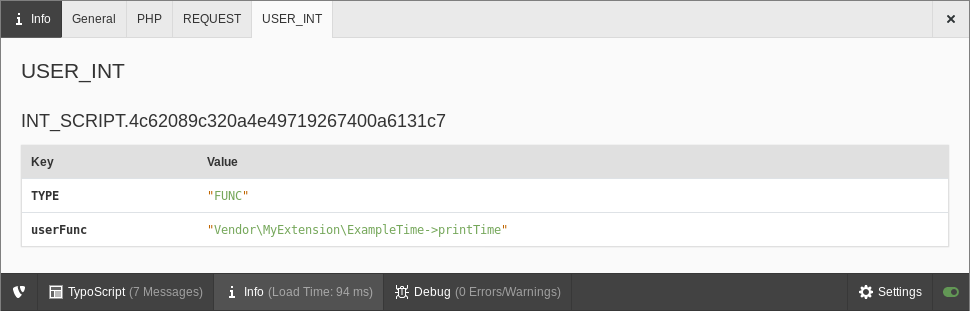
\includegraphics[width=0.90\linewidth]{ChangesForIntegrators/88441-ShowUserIntObjectsInAdminPanel.png}
	\end{figure}

\end{frame}

% ------------------------------------------------------------------------------
